 
% =============================================
% ================= PREÁMBULO =================
% =============================================

\documentclass[12pt,a4paper]{article}
\usepackage[utf8]{inputenc}
\usepackage[T1]{fontenc}        % Para Tildes
\usepackage[spanish,es-tabla]{babel}
\usepackage{graphicx}
\usepackage{cite}
\usepackage{minted}



\usepackage{multicol,multirow}
\usepackage{amsmath,mathtools}
\usepackage{amsfonts}
\usepackage{amssymb}
\usepackage{adjustbox}
\usepackage[europeanresistors]{circuitikz}
\usepackage{siunitx,enumitem}
\usepackage{pdfpages}       % Para importar páginas de un pdf 
\usepackage{booktabs}
\usepackage{physics}
\usepackage[bookmarks=true,colorlinks=true,linkcolor=black,citecolor=black,menucolor=black,urlcolor=black]{hyperref} 
\usepackage[left=2cm,right=2cm,top=2cm,bottom=2cm]{geometry} 
\usepackage{float}      % Para ubicar las tablas y figuras justo después del texto
\usepackage{pdfpages}
\usepackage{svg}
\usepackage[numbered,framed]{matlab-prettifier}
\usepackage{filecontents}
\usepackage{dirtytalk}
\usepackage{cancel}

\newcommand\Ccancel[2][black]{\renewcommand\CancelColor{\color{#1}}\cancel{#2}}

\usepackage{tikz}

\newcommand{\lapt}{
  \begin{tikzpicture}[baseline=-0.5ex]
    \draw (0,0) circle [radius=0.5ex];
    \draw (0.5ex,0) -- (3.5ex,0); 
    \draw[fill] (4ex,0) circle [radius=0.5ex];
  \end{tikzpicture} 
  \hspace{0.2cm}
}

\newcommand{\ilapt}{
  \begin{tikzpicture}[baseline=-0.5ex]
    \draw[fill] (0,0) circle [radius=0.5ex];
    \draw (0.5ex,0) -- (3.5ex,0);
    \draw (4ex,0) circle [radius=0.5ex];
  \end{tikzpicture}
   \hspace{0.2cm}
}


% =============================================
% ================= DOCUMENTO =================
% =============================================

\begin{document} 
% =============================================
% ================= PORTADA ===================
% =============================================

\begin{titlepage}
  \centering
  {\LARGE Universidad de Costa Rica \par} % Nombre de la universidad
  {\Large Facultad de Ingeniería \par} % Facultad
  {\Large Escuela de Ingeniería Eléctrica \par} % Escuela
  {\Large IE0347 $-$ Señales y Sistemas II \par} % Escuela
  \vspace{2cm}
  
  \includegraphics[width=0.3\textwidth]{IMG/imagen1.png} % Cambia "ruta/a/tu/logo" por la ruta a tu archivo de imagen del logo
  \vspace{1cm}

  {\huge\bfseries Tarea diagramas de bloques \par} % Título del documento
  \vspace{2cm}
  
  {\Large\ Estudiante: Ruiz Sánchez Junior Alfonso B97026 \par} % Nombre del estudiante
  {\Large\ Profesor: Helber Meneses Navarro \par} % Nombre del profesor
  \vfill
  
  {\large 7 de Mayo del 2024 \par} % Fecha
  \vspace*{\fill}
  
\end{titlepage}

\thispagestyle{empty} % No numerar la portada

\renewcommand{\thepage}{\roman{page}}
\newpage

%%%%%%%%%%  
\renewcommand{\thepage}{\arabic{page}} 
\setcounter{page}{1}

\newpage
\section{Simulación de circuito mediante diagrama de bloques}


\begin{figure}[H]\label{fig:rectificador}
    \centering
    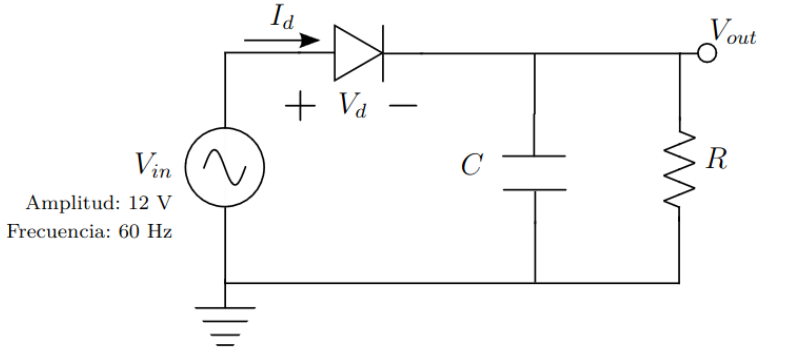
\includegraphics[width=0.5\textwidth]{imagenes/circuito.png}
    \caption{Circuito rectificador}
\end{figure}

Valores:

\begin{equation*}
    n = 1 \hspace{1cm} R = 100\, k \Omega \hspace{1cm} I_s = 10 ^ {-12} \, A
    \hspace{1cm} C = 1\, \mu F
\end{equation*}

\begin{equation*}
   q = 1, 602176565 \times 10 ^ {-19} C
   \hspace{1cm}
   k = 1, 3806488 \times 10^ {23} \dfrac{J}{K}
\end{equation*}

Equaciones: \\

\begin{multicols}{2}

\begin{equation*}
    I_d = I_s \left(e ^{
        \frac{V_d}{nV_T}
        } - 1 \right)
\end{equation*}

\begin{equation*}
V_T = \frac{kT}{q}    
\end{equation*}

\end{multicols}

Modelo del sistema:

\begin{equation*}
    C\:\frac{dV_{out}\left(t\right)}{dt}+\frac{1}{R}V_{out}\left(t\right)
    =
    I_s \left(e ^{
    \frac{V_{in}\left(t\right)-V_{out}\left(t\right)}
    {nV_T}
    } - 1 \right)
\end{equation*}

\begin{equation}
    \frac{dV_{out}(t)}{dt} = \frac{I_s}{C} \left( e^{\frac{V_{in}(t) - V_{out}(t)}{nV_T}} - 1 \right) - \frac{1}{RC}V_{out}(t)
\end{equation}

\subsection{Diagrama en simulink}

\begin{figure}[H]\label{fig:Diagrama}
    \centering
    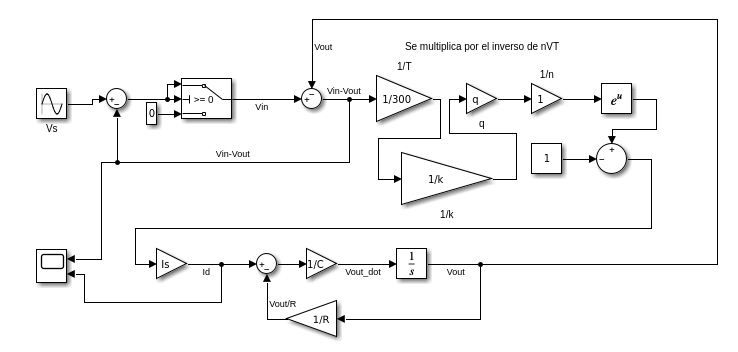
\includegraphics[width=0.9\textwidth]{imagenes/Diagrama.png}
    \caption{Diagrama generado en simulink}
\end{figure}

Mediante la ecuación (1) se realiza el estado Vout\_dot para después integrarlo, obtener vout 
y retroalimentarlo en donde es necesario.

\subsection{Resultados}
\begin{figure}[H]\label{fig:voutVin}
    \centering
    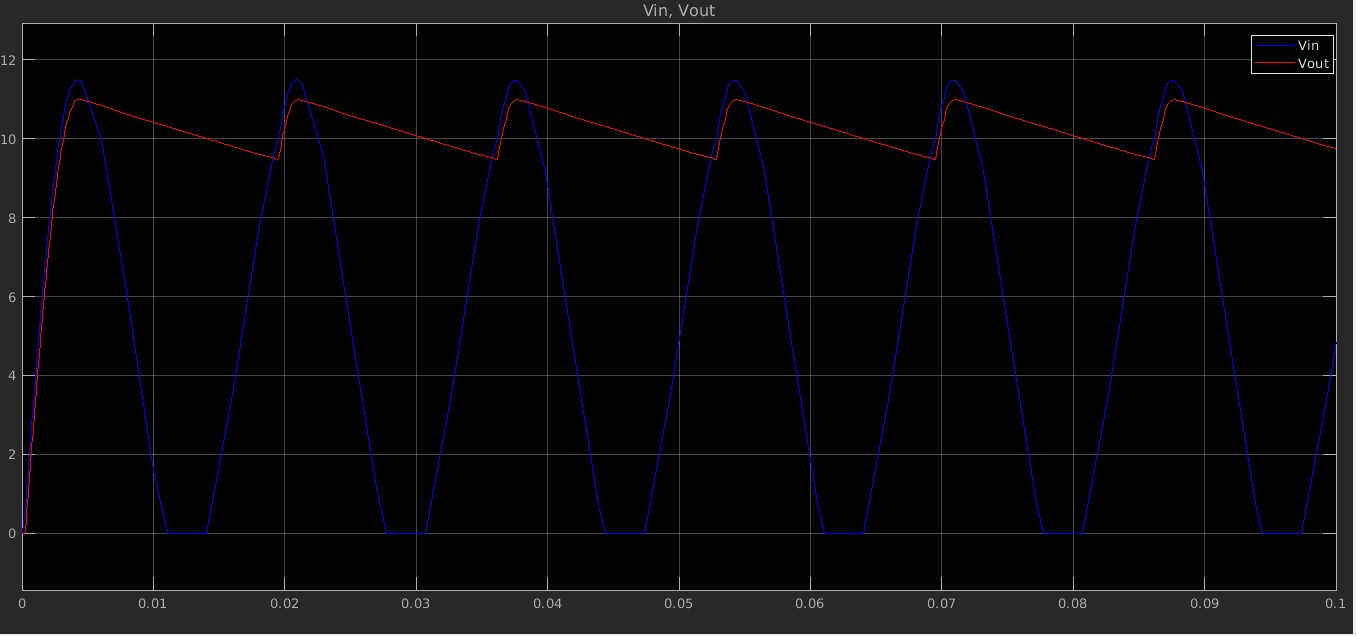
\includegraphics[width=0.9\textwidth]{imagenes/VoutVin.jpg}
    \caption{Tensión de entrada del circuito y tensión de salida
    del circuito vs tiempo}
\end{figure}

Se puede notar que efectivamente la tensión de entrada es de media onda, 
la tensión de salida es una onda rectificada con un rizado notable.
Los resultados son los esperados.

\begin{figure}[H]\label{fig:vd}
    \centering
    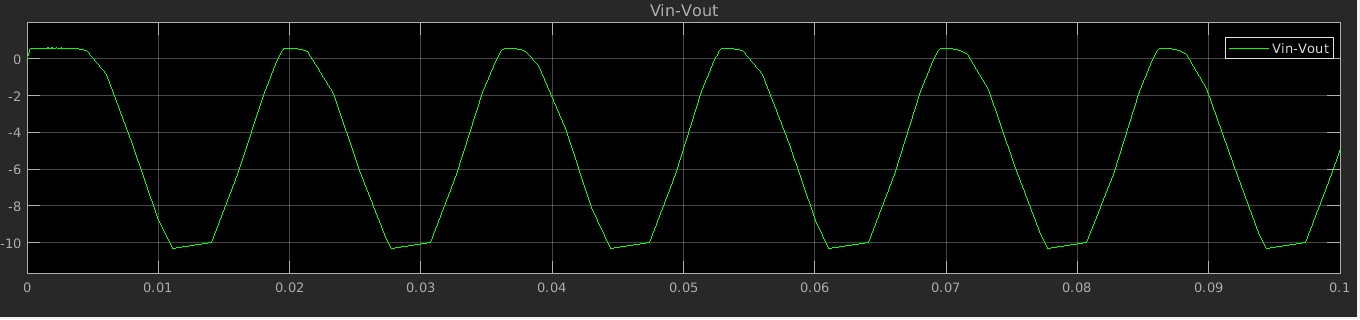
\includegraphics[width=0.9\textwidth]{imagenes/VD.jpg}
    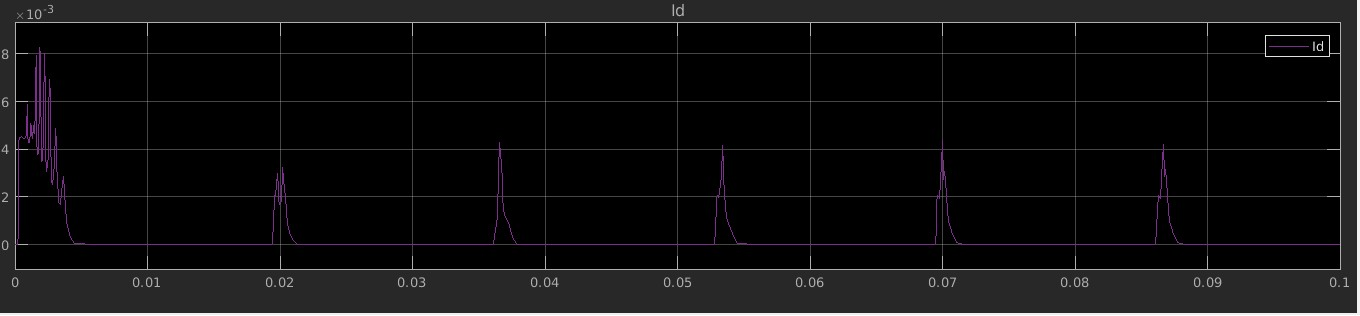
\includegraphics[width=0.9\textwidth]{imagenes/ID.jpg}
    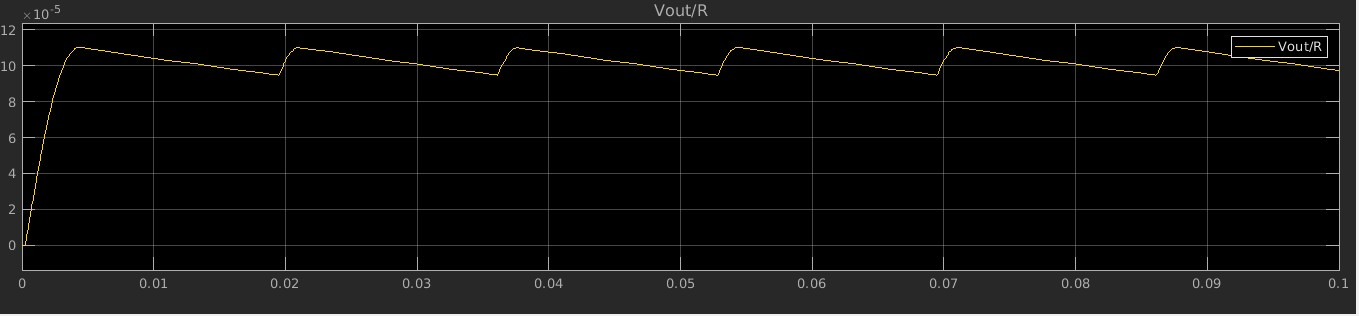
\includegraphics[width=0.9\textwidth]{imagenes/IR.jpg}
    
    \caption{Tensión del diodo y corriente del diodo vs tiempo}
\end{figure}

La tensión del diodo oscila, pero las zonas significativas son cuando la 
tensión de este es mayor a cero, se puede notar que en esos momentos 
hay corriente atravezando el diodo. Mientras que en las zonas en las que no hay
corriente es debido a que la tensión en el diodo es negativa por lo qué este no
se polariza, además la corriente de la carga tiene el mismo comportamiento que
la tensión de salida, pero con magnitud 100k veces menor,
es por esto que los resultados son los esperados.

\newpage
\section{Función de transferencia de un diagrama de bloques
 utilizando álgebra de bloques }

 \begin{figure}[H]\label{fig:DB}
    \centering
    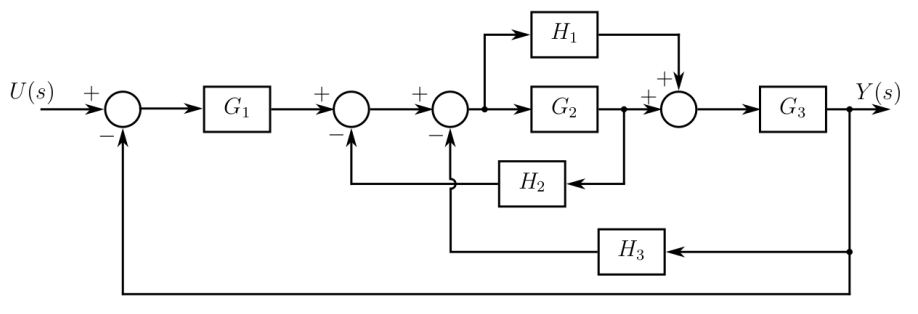
\includegraphics[width=\textwidth]{imagenes/bloques.png}
    \caption{Diagrama de bloques del problema 02}
 \end{figure}

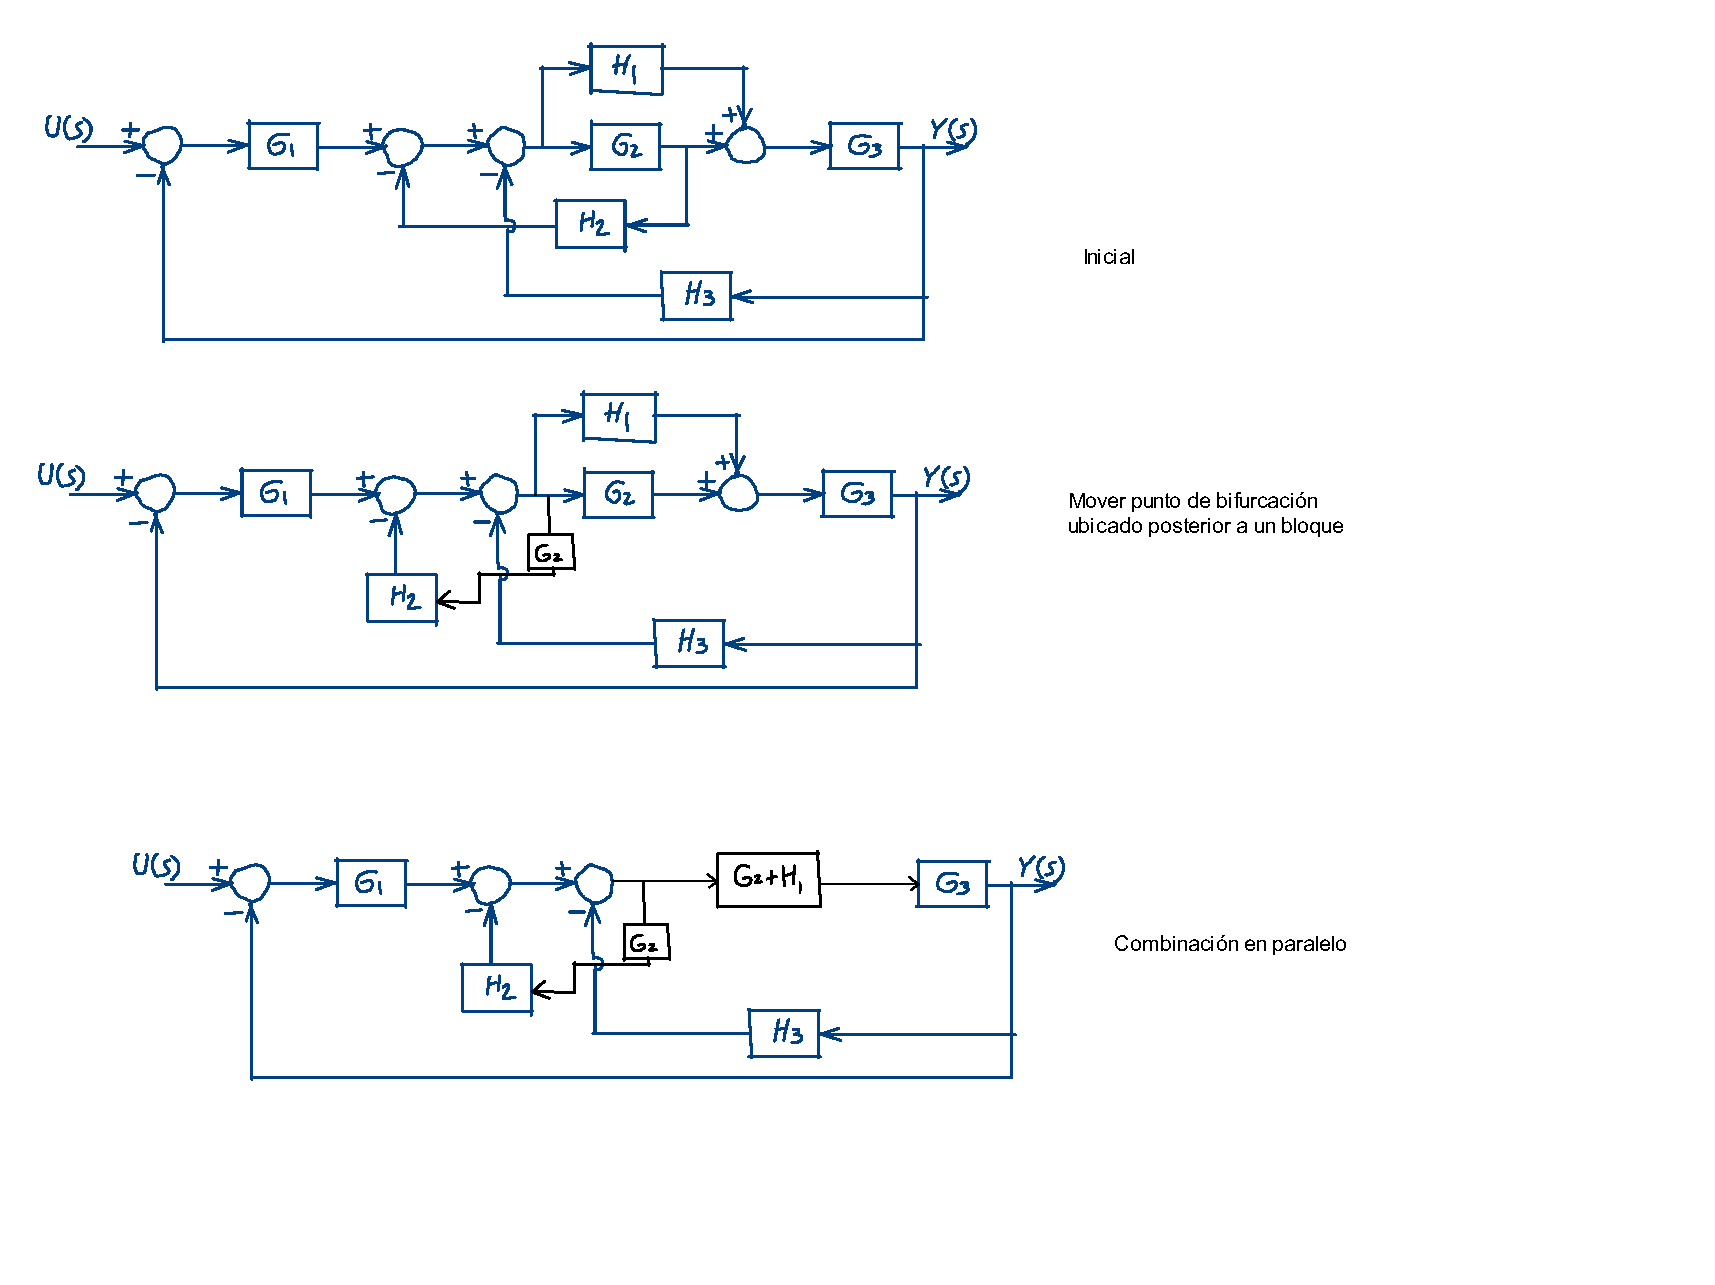
\includepdf[pages=-]{problema2.pdf}


\end{document}
